\documentclass[a4paper]{article}

%% Language and font encodings
\usepackage[english]{babel}
\usepackage[utf8x]{inputenc}
\usepackage[T1]{fontenc}

%% Sets page size and margins
\usepackage[a4paper,top=3cm,bottom=2cm,left=3cm,right=3cm,marginparwidth=1.75cm]{geometry}

%% packages for tables
\usepackage{booktabs}

%% Useful packages
\usepackage{amsmath}
\usepackage{graphicx}
\usepackage[colorinlistoftodos]{todonotes}
\usepackage[colorlinks=true, allcolors=blue]{hyperref}
\usepackage[numbers,sort&compress]{natbib} 
\usepackage{float}	% used for fix the location of tables and graphics
\newcommand{\upcite}[1]{\textsuperscript{\cite{#1}}}
\newcommand{\topcaption}{%
	\setlength{\abovecaptionskip}{0pt}%
	\setlength{\belowcaptionskip}{10pt}%
	\caption}   % 表格上标题修改

%_____________________________________________

\title{Numerical Methods Solving ODE}
\author{
	Ye Fengyang (3180111549) \\
	Tang Yuan (3180111524)   \\
	Du Yiqing (3180112696)   \\
	Shu Yue (3180111518)     \\
	Li Ruiqi (3180111638)
}

\begin{document}
	
	\maketitle
	
	%_____________________________________________
	\section{Introduction}
	
	At present, Ordinary Differential Equation (ODE) has been widely used in many aspects such as physics, biology and economics. In practical problems, it is particularly important to find the solution of ordinary differential equations. Despite the analytical solution can find the accurate answer, in some practical problems either it is hard to find the analytic solutions or the solving process is too complicated. In this case, it is extremely important to find the numerical solution of ODE by some methods (such as Euler method, Runge-Kutta method and Adams method). In this report, three methods -- Euler method, Runge-Kutta method and Adams method—have been compared in the process of solving the two practical problems.
	
	%_____________________________________________
	
	\subsection{Euler’s Method}
	
	Euler’s method mainly consists of three methods—the Forward Euler’s Method, the Backward Euler’s Method and the Improved Euler’s Method.
	The Forward Euler’s Method approximate the value of $\Phi(t)$ in the region $[t_n, t_{n+1}]$ of the curve by the line through $(t_n, y_n)$ with the slope $f(t_n, y_n)$. The formula is in the form:
	
	\begin{equation}\label{eq.1}
		y_{n+1} = y_n + hf(t_n, y_n), \enspace n = 0,1,2,...
	\end{equation}
	
	The Backward Euler’s Method approximate the value of $\Phi(t)$ in the region $[t_n, t_{n+1}]$ of the curve by the line through $(t_n, y_n)$ with the slope $f(t_{n+1}, y_{n+1})$. The formula is in the form:
	
	\begin{equation}\label{eq.2}
		y_{n+1} = y_n + hf(t_{n+1}, y_{n+1}), \enspace n = 0,1,2,...
	\end{equation}	

	The Improved Euler’s Method approximate the value of $\Phi(t)$ in the region $[t_n, t_{n+1}]$ of the curve by the line through $(t_n, y_n)$ with the slope $\frac{1}{2} (f(t_n) + f(t_{n+1}))$. The formula is in the form:
	
	\begin{equation}\label{eq.3}
		y_{n+1} = y_n + {h \over 2}(f(t_n) + f(t_n + h))), \enspace, n = 0,1,2,...
	\end{equation}	
	
	%_____________________________________________
	
	\subsection{The Runge-Kutta Method}
	
	The Runge-Kutta Method is similar to the Euler’s Method, however, in this method, we try to find the slope with a few more points on the region $[t_n, t_{n+1}]$, then taking a weighted average of the slope values at these points, and using the resulting value as the approximate slope $k$.
	In this report we discuss the fourth-order four-stage Runge-Kutta method. The formula is in the form:
	
	\begin{equation}\label{eq.4}
		y_{n+1} = y_n + h(\frac{k_{n1} + 2k_{n2} + 2k_{n3} + k_{n4}}{6}), \enspace n = 0, 1, 2,...
	\end{equation}

	Where
	
	\begin{align} \nonumber
		k_{n1} &= f(t_n, y_n), \\ \nonumber
		k_{n2} &= f(t_n + {1 \over 2}h, y_n + {1 \over 2}hk_{n1}), \\ \nonumber
		k_{n3} &= f(t_n + {1 \over 2}h, y_n + {1 \over 2}hk_{n2}), \\ \nonumber
		k_{n4} &= f(t_n + h, y_n + hk_{n3}), \\ \nonumber
	\end{align}
	
	%_____________________________________________
	
	\subsection{Adam’s Method}
	
	Adam’s Method makes use of a polynomial $P_k(t)$ of degree $k$ to approximate $phi'(t)$ and evaluates the integral of $phi'(t)$.
	Second-order Adams-Bashforth formula is
	
	\begin{equation}\label{eq.6}
		y_{n+1} = y_n + {3 \over 2}hf_n - {1 \over 2}f_{n-1}, \  n = 0,1,2,...
	\end{equation}
	
	Fourth-order Adams-Bashforth formula is
	
	\begin{equation}\label{eq.7}
		y_{n+1} = y_n + {h \over 24}(55f_n - 59f_{n-1} + 37f_{n-2} - 9f_{n-3}), \  n = 0,1,2,...
	\end{equation}
	
	%_____________________________________________
	
	\section{Analytical Solution}
	
	\subsection{Problem 1}
	
	Before using numerical method to calculate, we try to use analytical method to calculate the accurate answer.
	Substitute $y(t) = \sum_{n=0}^{\infty} a_n t^n$ into the ODE and equate coefficients. Then we can get
	
	\begin{equation}
		(n+1)a_{n+1}-a_{n-1} = 
			\begin{cases}
				\sum_{k=0}^{n-k}, & \text{$n \neq 2$} \\
				2a_0a_n + a_1^2 + 1, & \text{$n = 2$}
			\end{cases}
	\end{equation}

	Which is hard to calculate
	
	%_____________________________________________
	
	\subsection{Problem 2}
	
	Similar to Problem 1, we calculate analytical solution at first.
	We also substitute $y(t) = \sum_{n=0}^{\infty} a_n t^n$ into the ODE.
	
	%_____________________________________________
	
	\section{Numerical Solution}
	
	\subsection{Problem 1}
	
	Since $y' = y^2 + ty + t^2 = (y + {1 \over 2}t)^2 + {3 \over 4}t^2 \geq 0$, so $y = f(t)$ will increase in its domain.
	
	\begin{figure}[H]
		\centering
		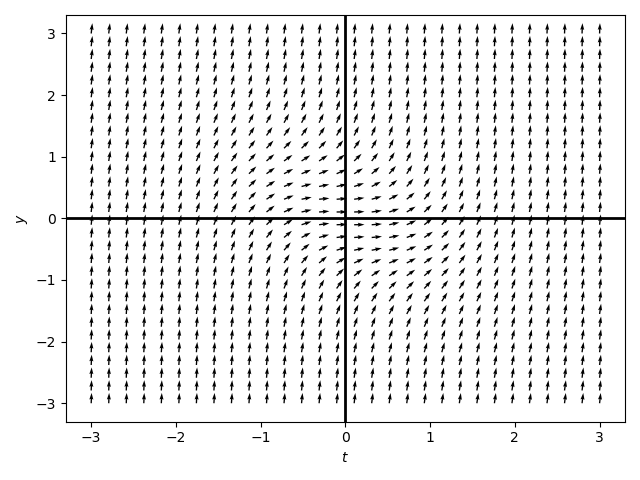
\includegraphics[width=8cm]{img/slope_field1.png}
		\caption{\label{fig:slope_field1} The slope field of $f(t, y)$ of Problem 1}
	\end{figure}

	We can construct a slope field as \autoref{fig:slope_field1}.
	
	We can estimate that there might be two vertical asymptotes, $a_1$, $b_1$. Since the slope of the vector tends to be infinity near $t=-2$ and $t=1$, so we can have a try: let $a_1$ very close to -2 and $b_1$ very close to 1 to find accurate vertical asymptotes.
	
	\begin{table}[H]
		\centering
		\resizebox{\textwidth}{!}{%
			\begin{tabular}{@{}ccccccccc@{}}
				\toprule
				& \multicolumn{2}{c}{\textbf{Euler Implicit}} & \multicolumn{2}{c}{\textbf{Euler Explicit}} & \multicolumn{2}{c}{\textbf{Euler Improved}} & \multicolumn{2}{c}{\textbf{Euler Trapezium}} \\ \midrule
				\textbf{$h$} & \textbf{$a_1$}          & \textbf{$b_1$}          & \textbf{$a_1$}          & \textbf{$b_1$}          & \textbf{$a_1$}          & \textbf{$b_1$}          & \textbf{$a_1$}           & \textbf{$b_1$}          \\
				\hline 
				0.01       & -2.07                & 0.82                 & -2.26                & 1                    & -2.17                & 0.91                 & -2.11                 & 0.85                 \\
				0.005      & -2.09                & 0.83                 & -2.195               & 0.935                & -2.15                & 0.885                & -2.115                & 0.855                \\
				0.001      & -2.115               & 0.853                & -2.137               & 0.875                & -2.126               & 0.864                & -2.1201               & 0.859                \\
				0.0005     & -2.118               & 0.856                & -2.129               & 0.8675               & -2.1235              & 0.8615               & -2.1206               & 0.8591               \\
				0.0002     & -2.1196              & 0.8578               & -2.1242              & 0.8624               & -2.1218              & 0.86                 & -2.1208               & 0.8592               \\
				0.0001     & -2.1202              & 0.8584               & -2.1225              & 0.8607               & -2.1212              & 0.85964              & -2.1209               & 0.8592               \\ \bottomrule
			\end{tabular}%
		}
	\caption{Using Euler Method to Determine $t$ When $y$ is infinity}
	\label{tab:euler_inf}
	\end{table}

	%____________________________________________
	
	\subsubsection{The Euler Method}

	When $h=0.01$, vertical asymptotes are not stable. As $h$ is decreasing, $a_1$, $b_1$ gradually reach to a stable value. When $h=0.0001$, the value of $a_1$, $b_1$ calculated by these four methods is absolutely close. Digitally, we can solve that $a_1=-2.1212$, $b_1=0.8594$.
	
	To be more vivid, we can basically draw $y=f(t)$ as \autoref{fig:ivp1_sol}.
	
	\begin{figure}[H]
		\centering
		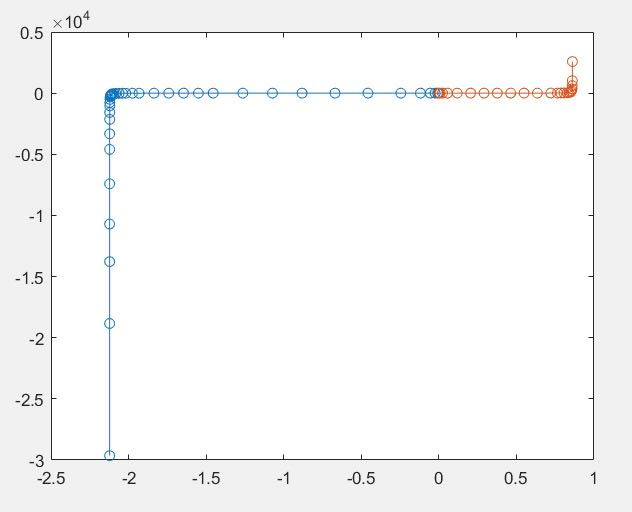
\includegraphics[width=8cm]{img/ivp1_sol.png}
		\caption{\label{fig:ivp1_sol} The Solution of Problem 1}
	\end{figure}
	
	%_____________________________________________
	
	\subsubsection{The Runge-Kutta Method}
	
	The stable value of $a_1$, $b_1$ can be got when $h=0.0001$. RK 4th has more accuracy, but in this particular problem, compared with RK 3rd, it doesn’t fully manifest. When $h=0.01$ or $0.005$, the value of $a_1$, $b_1$ is not so accurate, but not far from stable value. Therefore, we can solve $a_1=-2.1209$, $b_1= 0.8591$.
	
	\begin{table}[H]
		\centering
		\resizebox{220pt}{!}{%
			\begin{tabular}{@{}ccccc@{}}
				\toprule
				& \multicolumn{2}{c}{\textbf{RK 3rd}} & \multicolumn{2}{c}{\textbf{RK 4th}} \\ \midrule
				\textbf{h} & \textbf{a1}      & \textbf{b1}      & \textbf{a2}      & \textbf{b2}      \\
				0.01       & -2.15            & 0.89             & -2.14            & 0.88             \\
				0.005      & -2.135           & 0.875            & -2.13            & 0.87             \\
				0.001      & -2.124           & 0.862            & -2.123           & 0.861            \\
				0.0005     & -2.122           & 0.8605           & -2.122           & 0.86             \\
				0.0002     & -2.1212          & 0.8596           & -2.121           & 0.8594           \\
				0.0001     & -2.121           & 0.8592           & -2.1209          & 0.8591           \\ \bottomrule
			\end{tabular}%
		}
		\caption{Using Runge-Kutta Method to Determine t When y is infinity}
		\label{tab:rk_inf}
	\end{table}
	
	%_____________________________________________
	
	\subsubsection{The Adams Method}
	
	For Adams Bashforth method, when $h$ is not small enough, the value of $a_1$, $b_1$ can’t be stable. Just when $h$ is smaller than the level of $10^{-3}$, $a_1$, $b_1$ will tend to be stable. However, for Adams Molton method, no matter what value $h$ is, in other words, for $h=0.01,0.005,0.001,0.0005,0.0002,0.0001$, in each condition, the value of $a_1$, $b_1$ have little difference. So it can be concluded that Adams Monlton has more accuracy than Adams Bashforth. As a result, we can solve $a_1=-2.1207$, $b_1=0.8588$.
	
	\begin{table}[H]
		\centering
		\resizebox{220pt}{!}{%
			\begin{tabular}{@{}ccccc@{}}
				\toprule
				& \multicolumn{2}{c}{\textbf{Adams-Bashforth}} & \multicolumn{2}{c}{\textbf{Adams-Monlton}} \\ \midrule
				\textbf{h} & \textbf{a1}           & \textbf{b1}          & \textbf{a2}          & \textbf{b2}         \\
				\hline
				0.01       & -2.21                 & 0.95                 & -2.12                & 0.85                \\
				0.005      & -2.17                 & 0.905                & -2.1201              & 0.855               \\
				0.001      & -2.13                 & 0.868                & -2.1202              & 0.858               \\
				0.0005     & -2.1255               & 0.8635               & -2.1205              & 0.8585              \\
				0.0002     & -2.1226               & 0.8608               & -2.1206              & 0.8587              \\
				0.0001     & -2.1216               & 0.8598               & -2.1207              & 0.8588              \\ \bottomrule
			\end{tabular}%
		}
		\caption{Using Adams Method to Determine t When y is infinity}
		\label{tab:adams_inf}
	\end{table}

	%_____________________________________________
	
	%_____________________________________________
	
	\subsection{Problem 2}
	
	% TODO
	
	%_____________________________________________
	
	\section{Methods}
	%次标题
	\subsection{AAA}
	%更次标题
	\subsubsection{BBB}

	\autoref{eq.10} is a equation example.
	
	
	\begin{equation}
		RMSE(k)=RMSE(k)=\sqrt{\frac{\Sigma^{100}_{i=1}(\hat{x}+1)^2+(\hat{x_2}+1)^3}{k}}
	\end{equation}\label{eq.10}
	
	An other example about equation.
	Let $f(x)$ be defined by the formula$$f(x)=3x^2+x-1$$ which is a polynomial of 2.
	
	%_____________________________________________
	
	\section{byebye}
	
	%插入文献
	CN DOTA, BEST DOTA!\upcite{Menard2002Applied,Peduzzi1996A,Compton2002HABITAT}
	
	%插入表格
	\begin{table}[http]
		%调整行距
		\renewcommand{\arraystretch}{2}
		%表格剧中
		\centering
		%设置表标题在上面
		\topcaption{imlulation}
		%设置label
		\label{tab}
		%表格具体内容
		\begin{tabular}{ccc}
			\hline \hline
			good & bad & total  \\ \hline
			26   & 26  & 2559   \\
			3    & d   & dd     \\ \hline \hline
		\end{tabular}
	\end{table}
	
	%_____________________________________________
	
	%插入文献,IEEEtran为格式,sample为.bib文件名
	\bibliographystyle{IEEEtran}
	\bibliography{sample}
	
\end{document}